    Наиболее простым видом столкновительно-индуцированных спектров являются трансляционные спектры, порождаемые смесью двух благородных газов при низком давлении, где доминируют бинарные столкновения. При более высоких давлениях будут случаться столкновения с участием трех и более атомов, которые будут видоизменять форму спектра поглощения. На рис. \ref{pic-two-atom-experiment} приведены примеры экспериментальных столкновительно-индуцированных спектров поглощения в дальней ИК области систем He$-$Ar, Ne$-$Ar и Ar$-$Kr \cite{frommhold}. Было экспериментально подтверждено, что интенсивность поглощения линейно зависит от произведения плотностей газов $\rho_1 \rho_2$, что говорит о том, что спектр порождается парами разных атомов. Отклонение от линейной зависимости будет говорить о том, что при данных концентрациях существенный вклад вносят многочастичные столкновения. Спектры, изображенные на рис \ref{pic-two-atom-experiment}, сняты при разных концентрациях от 60 амага (He$-$Ar) до 200 амага (Ar$-$Kr).  

\begin{figure}[H]
    \centering
    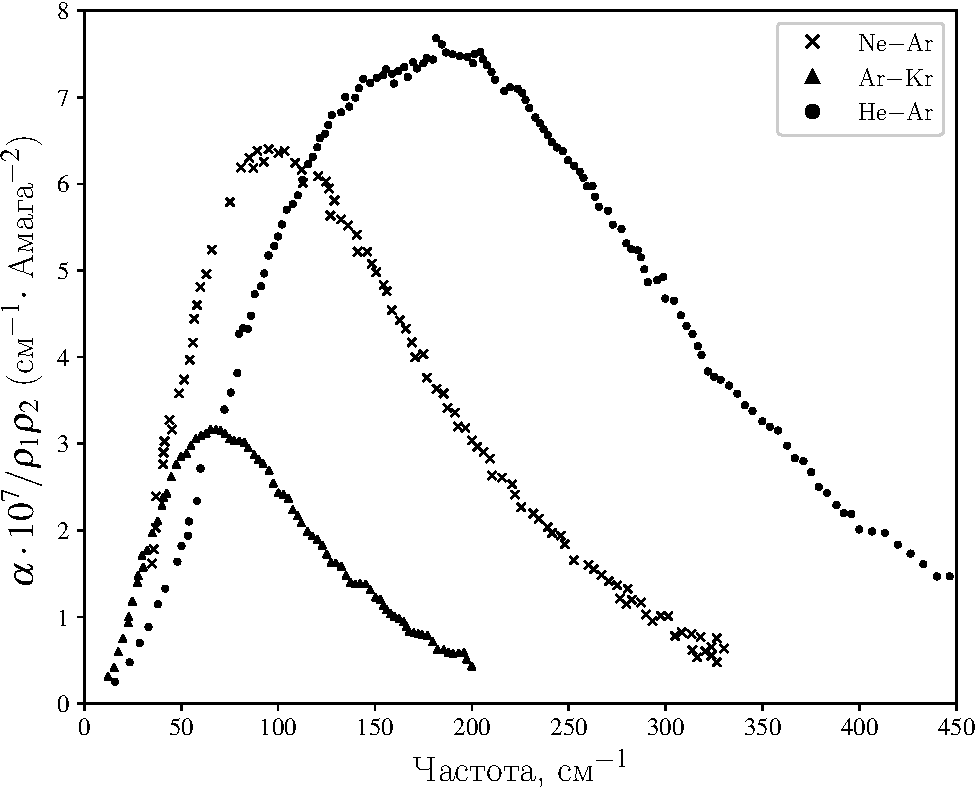
\includegraphics[width=0.7\linewidth]{./pictures/twoatom_experiment/experiment_diatom_spectra-crop.pdf}
    \label{pic-two-atom-experiment}
    \caption{Экспериментальные спектры бинарного поглощения систем гелий$-$аргон, неон$-$аргон и аргон$-$криптон при комнатной температуре \cite{frommhold}}
\end{figure}

В работе \cite{kranendonk1973} авторы разрабатывают формализм расчета столкновительно-индуцированного спектра в приближении бинарных столкновений. Авторы рассматривают систему, состояющую из молекулы $H_2$, возмущенной атомами $Ar$. Вращательное движение молекулы $H_2$ исключено из рассмотрения -- обе сталкивающихся молекулы рассматриваются как безструктурные сферически-симметричные частицы. \par
    Спектральная функция, определяющая профиль спектра поглощения, связана с функцией автокорреляции суммарного дипольного момента системы преобразованием Фурье
\begin{gather}
    J(\omega) = \intty \mean{ \bs{\mu}(0) \bs{\mu}(t) } e^{i \omega t} dt. \label{twoatom-spectral-function}
\end{gather} 
В приближении бинарных столкновений корреляционная функция суммарного дипольного момента становится 
\begin{gather}
    \mean{ \bs{\mu}(0) \bs{\mu}(t) } = N \mean{ \bs{\mu}_1(0) \bs{\mu}_1(t) },
\end{gather} 
%
где через $\bs{\mu_1}(t)$ обозначен дипольный момент индуцированный квадрупольным полем молекулы $H_2$ на атоме $Ar$, а $N$ -- количество рассматриваемых пар. Приведенную массу системы обозначают через $\mu$; вектор, соединяющий центр масс молекулы $H_2$ атомом $Ar$ -- через $\mathbf{R}$; потенциал взаимодействия -- через $V(R)$ $[$как уже говорилось, вращательное движение молекулы водорода не рассматривается, поэтому потенциал зависит только от расстояния между центрами масс $R$$]$. Автокорреляционную функцию дипольного момента приводят к виду 
\begin{gather}
    C(\tau) = \frac{N}{V} \lb \frac{\mu}{2 \pi k T} \rb^{3/2} \iint \bs{\mu}_1(\mathbf{R}) \cdot \bs{\mu}_1(\mathbf{R}(\tau)) \exp \lb -\frac{\mu \dot{\mf{R}}^2}{2 k T} \rb g_0(R) \, d \mathbf{R} \, d \dot{\mathbf{R}}, \label{kranendonk-correlation-function}
\end{gather}
%
где $\mathbf{R}(\tau)$ -- значение $\mathbf{R}$, вычисленное в момент времени $\tau$ путем расчета классической траектории, начальными условиями для которой взяты $\mf{R}$ и $\dot{\mf{R}}$, и $g_0(R)$ -- парная функция распределения (вероятность того, что между атомами расстояние $R$)
\begin{gather}
    g_0(R) = \exp \lb -\frac{V(R)}{kT} \rb.
\end{gather}

Выражение \eqref{kranendonk-correlation-function} неудобно для численного расчета, т.к. в нем имеется $R(\tau)$ для произвольного момента времени $\tau$. Для более эффективной вычислительной схемы предлагается переписать интегральное выражение \eqref{kranendonk-correlation-function} как интеграл по полным столкновительным траекториям. При этом будут рассматриваться только траектории рассеяния. В лабораторной системе отсчета энергия система может быть записана в виде
\begin{gather}
    E = \frac{1}{2} \mu \dot{\mf{R}}^2 + V(R).
\end{gather}
Траекторию рассеяния, которая имеет в момент времени $t$ радиус-вектор $\mf{R}$ и скорость $\dot{\mf{R}}$, может быть однозначно определена относительной скоростью $\mf{g}$ в момент времени $t = -\infty$, прицельным параметром $b$, углом, определяющим ориентацию плоскости столковения $\varepsilon$, и моментом времени $t_0$, в которое произошло столкновение. Применяя теорему Лиувилля
\begin{gather}
    d \mf{R} \, d\dot{\mf{R}} = g d(t - t_0) b db \, d\varepsilon \, d\mf{g},
\end{gather}
%
выражение \eqref{kranendonk-correlation-function} преобразуют к виду
\begin{gather}
    C(\tau) = \frac{N}{V} \lb \frac{\mu}{2 \pi k T} \rb^{3/2} \idotsint \bs{\mu}_1(t) \cdot \bs{\mu}_1(t + \tau) \, g \exp \lb - \frac{\mu \mf{g}^2}{2 k T} \rb b \, db \, d\varepsilon \, d \mf{g}. \label{correlation-function-kranendonk}
\end{gather}

Корреляцией двух функций $f$ и $g$, определенных на комплексной плоскости $\mathbb{C}$, называют функцию, определенную следующим интегралом
\begin{gather}
    C(\tau) = \intty f^{*}(t) g(\tau + t) dt,
\end{gather}
% 
где $*$ обозначает комплексное сопряжение. Обозначим через $F(\omega)$, $G(\omega)$ Фурье-образы функций $f(t)$, $g(t)$. Перепишем выражение для корреляции, представив функции через обратное преобразование Фурье от $F(\omega)$, $G(\omega)$, соответственно.
\begin{gather}
    C(\tau) = \intty \lsq \, \intty F^{*}(\omega) e^{-i \omega t} \frac{d \omega}{2 \pi} \rsq \lsq \, \intty G(\omega^\prime) e^{i \omega^\prime (\tau + t)} \frac{d\omega^\prime}{2 \pi} \rsq
\end{gather}

Осуществляя перестановку внутри интегрального выражения, приходим к следующему выражению 
\begin{gather}
    C(\tau) = \frac{1}{2\pi} \intty \intty F^*(\omega) G(\omega^\prime) e^{i \omega^\prime \tau} \lsq \, \intty e^{i (\omega^\prime - \omega) t} \frac{dt}{2 \pi} \rsq d\omega d\omega^\prime = \notag \\
    = \frac{1}{2\pi} \intty \inty F^*(\omega) G(\omega^\prime) e^{i \omega^\prime \tau} \delta \lb \omega^\prime - \omega \rb d\omega d\omega^\prime = \hat{F}^{-1} \Big[ F^*(\omega) G(\omega) \Big],
\end{gather}
%
где через $\hat{F}$ обозначен оператор преобразования Фурье. Если рассмотреть эту цепочку преобразований для автокорреляционной функции действительной функции $f(t)$, то приходим к теореме Винера-Хинчина \cite{frommhold}
\begin{gather}
    \hat{F} \Big[ C(\tau) \Big] = \Big\vert \hat{F}\Big[ f(t) \Big] \Big\vert^2. 
\end{gather}

Автокорреляционная функция дипольного момента распадается на сумму автокорреляционных функций его компонент
\begin{gather}
    C(\tau) = \intty \bs{\mu}_1(t) \bs{\mu}_1(t + \tau) dt = \sum_{\alpha = x, y, z} \intty \mu_1^\alpha(t) \mu_1^\alpha(t + \tau) dt = C_x(\tau) + C_y(\tau) + C_z(\tau).
\end{gather}

Следовательно, преобразование Фурье от автококорреляционной функции дипольного момента представляет собой сумму квадратов преобразований Фурье от компонент дипольного момента
\begin{gather}
    \hat{F}\Big[ C(\tau) \Big] = \sum_{\alpha = x,y,z} \hat{F} \Big[ C_\alpha(\tau) \Big] = \sum_{\alpha=x,y,z} \Bigg\vert \intty \mu_1^\alpha(t) e^{-i\omega t} dt \Bigg\vert^2,
\end{gather}
% 
что для краткости обозначают 
\begin{gather}
    \hat{F} \Big[ C(\tau) \Big] = \Bigg\vert \intty \bs{\mu}_1(t) e^{-i\omega t} dt \Bigg\vert^2.
\end{gather}

Итак, преобразование Фурье от автокорреляционной функции \eqref{correlation-function-kranendonk} дает спектральную функцию  
\begin{gather}
    J(\omega) = \frac{N}{V} \lb \frac{\mu}{2 \pi k T} \rb^{3/2} \idotsint \Bigg\vert \intty \bs{\mu}_1(t) e^{-i \omega t} dt \Bigg\vert^2 \, \exp \lb -\frac{\mu g^2}{2 k T} \rb b \, db \, d \varepsilon \, 4 \pi g^3 dg.
\end{gather}

\section{Корреляционная функция в системе отсчета, связанной с плоскостью движения}

Рассмотрим движение двух атомов в неподвижной декартовой системе координат. Обозначим через $m_1$, $m_2$ массы атомов, через $\mf{r}_1$, $\mf{r}_2$ -- радиус-векторы атомов. После отделения центра масс лагранжиан системы равен 
\begin{gather}
    \mL = \frac{\mu \dot{\mf{r}}^2}{2} - U( r ),
\end{gather}
где через $\mu$ обозначена приведенная масса атомов, а вектор $\mf{r}$ описывает $\mf{r}_1 - \mf{r}_2$. \par
Для перехода к гамильтониану, выразим обобщенные импульсы системы
\begin{gather}
    \mf{p} = \frac{\partial \mL}{\partial \dot{\mf{r}}} = \mu \dot{\mf{r}}.
\end{gather}
Таким образом, гамильтониан системы равен
\begin{gather}
    \mH = \frac{\mf{p}^2}{2\mu} + U( r ).
\end{gather}

Рассмотрим усреднение некоторой функции $f(\mf{r}, \mf{p})$ по фазовому пространству двухатомной системы. 
\begin{gather}
    \mean{f} = \idotsint f(\mf{r}, \mf{p}) \exp \lb -\frac{\mH(\mf{r},\mf{p})}{kT} \rb d \mf{r} \, d\mf{p} \label{two-atom-mean}
\end{gather}

Известно, что в отсутствии внешнего момента сил движение двухатомной системы происходит в плоскости, перпендикулярной вектору углового момента \cite{goldstein}. Следовательно, движение системы можно описать при помощи полярных координат $r, \psi$ в плоскости, и соответствующих обобщенных скоростей $\dot{r}$, $\dot{\psi}$. Кроме того, опишем ориентацию плоскости при помощи пары углов $\Phi$, $\Theta$. Целью нашего рассмотрения будет нахождение выражений, позволяющих производить усреднение функции по фазовому пространству, пользуясь тем, что движение системы ограничено в плоскости. \par
    Введем систему координат так, чтобы плоскость движения двухатомной системы совпадала с плоскостью $OXY$ введенной системы. Тогда координаты частицы с приведенной массой будут равны $\lc r \cos \psi, r \sin \psi, 0 \rc$. Лагранжиан системы равен
\begin{gather}
    \mL = \frac{\mu}{2} \lb \dot{r}^2 + r^2 \dot{\theta}^2 \rb - U(r). \label{two-atom-plane-lagrangian}
\end{gather}

Перевод координат между системами можно осуществить при помощи ортогональной матрицы вращения $\bbS$ \cite{goldstein}. В данном случае нам достаточно лишь двух углов, связь между координатами лабораторной системы $\mf{r} = \lc x, y, z \rc$ и полярными координатами на плоскости определена следующим соотношением
\begin{gather}
    \begin{bmatrix}
        x \\ y \\ z
    \end{bmatrix} = \bbS_\Phi^{-1} \bbS_\Theta^{-1} 
    \begin{bmatrix}
        r \cos \psi \\ r \sin \psi \\ 0
    \end{bmatrix}, \label{two-atoms-coordinate-transformation}
\end{gather}
% 
где матрицы поворота $\bbS_\Phi$, $\bbS_\Theta$ определены равны
\begin{gather}
    \bbS_\Phi = 
    \begin{bmatrix}
        \cos \Phi & \sin \Phi & 0 \\
       -\sin \Phi & \cos \Phi & 0 \\
      0 & 0 & 1
    \end{bmatrix}, \quad
    \bbS_\Theta = 
    \begin{bmatrix}
        1 & 0 & 0 \\
        0 & \cos \Theta & \sin \Theta \\
        0 & -\sin \Theta & \cos \Theta
    \end{bmatrix}.
\end{gather}

Найдем якобиан замены переменных $\lc \mf{r}, \dot{\mf{r}} \rightarrow \lc r, \psi, \dot{r}, \dot{\psi}, \Phi, \Theta \rc$. Для этого раскроем матричное выражение \eqref{two-atoms-coordinate-transformation}, продифференцируем полученные выражения по времени, учитывая, что углы $\Phi$ и $\Theta$ не зависят от времени,  и составим матрицу якобиана. Координаты вектора $\mf{r}$ связаны со вторым набором координат следующими соотношениями 
\begin{gather}
    \left\{
        \begin{aligned}
            x &= r \cos \psi \cos \Phi - r \sin \psi \sin \Phi \cos \Theta \\
            y &= r \cos \psi \sin \Phi + r \sin \psi \cos \Phi \cos \Theta \\
            z &= r \sin \psi \sin \Theta
        \end{aligned}
    \right.
\end{gather}

Дальнейшие выкладки приводить не будем, якобиан замены переменных получается следующий
\begin{gather}
    \text{Jac} = \Bigg\vert \frac{\partial \lsq x, y, z, \dot{x}, \dot{y}, \dot{z} \rsq}{\partial \lsq r, \psi, \dot{r}, \dot{\psi}, \Phi, \Theta \rsq} \Bigg\vert = r^4 \dot{\psi} \sin \Theta.
\end{gather}

Рассмотрим элемент фазового объема $\Gamma = d\mf{r} \, d\mf{p}$ в лабораторной системе координат. В лагранжевых переменных элемент может быть переписан как $\Gamma = \mu^3 d\mf{r} \, d\dot{\mf{r}}$. Затем перейдем к системе координат, связанной с плоскостью 
\begin{gather}
    \Gamma =  \mu^3 r^4 \dot{\psi} \sin \Theta \, dr \, d\psi \, d\dot{r} \, d\dot{\psi} \, d\Phi \, d\Theta. \label{two-atom-phase-space-element}
\end{gather}
Обобщенные импульсы, сопряженные координатам $r$ и $\psi$, могут быть получены из лагранжиана \eqref{two-atom-plane-lagrangian}
\begin{gather}
    p_r = \frac{\partial \mL}{\partial \dot{r}} = \mu \dot{r}, \quad p_\psi = \mu r^2 \dot{\psi}.
\end{gather}
Используя полученные уравнения, получаем следующее выражение для элемента фазового объема
\begin{gather}
    \Gamma = dr \, d\psi \, dp_r \, p_\psi \, dp_\psi \, \sin \Theta d\Theta \, d\Phi.
\end{gather}

В том случае, когда усредняемая функция $f(\mf{r}, \mf{p})$ не зависит от ориентации плоскости, можно проинтегрировать по углам $\Phi$, $\Theta$, в результате чего среднее значение \eqref{two-atom-mean} приходит к виду
\begin{gather}
    \mean{f} = 4 \pi \idotsint f(r, \psi, p_r, p_\psi) \exp \lb -\frac{p_r^2}{2\mu k T} - \frac{p_\theta^2}{2 \mu r^2 k T} - \frac{U(r)}{kT} \rb dr \, dp_r \, d\psi \, p_\psi \, dp_\psi. 
\end{gather}

Отметим, что импульс $p_\psi$ имеет физический смысл модуля углового момента, поэтому область интегрирования этого импульса составляет полуось $(0, +\infty)$, в то время как для радиального импульса -- вся прямая $(-\infty, +\infty)$.
